\begin{frame}{Tokenization: Why It Matters?}
  \begin{itemize}
    \item[\textcolor{red}{$\blacktriangleright$}] \textbf{Language $\neq$ Input}
    \begin{itemize}
      \item Text must be converted to numbers $\rightarrow$ tokens.
    \end{itemize}
    \vspace{0.7em}
    \item[\textcolor{red}{$\blacktriangleright$}] \textbf{Tokenization:}
    \begin{itemize}
      \item Splits text into manageable units.
      \item Balances granularity and vocabulary size.
    \end{itemize}
    \vspace{0.7em}
    \item[\textcolor{red}{$\blacktriangleright$}] \textbf{Good tokenizer =}
    \begin{itemize}
      \item Efficient sequence length
      \item High vocabulary coverage
      \item Robust across domains (code, multilingual, etc.)
    \end{itemize}
  \end{itemize}
\end{frame}


\begin{frame}{Machine Translation}
  \centering
  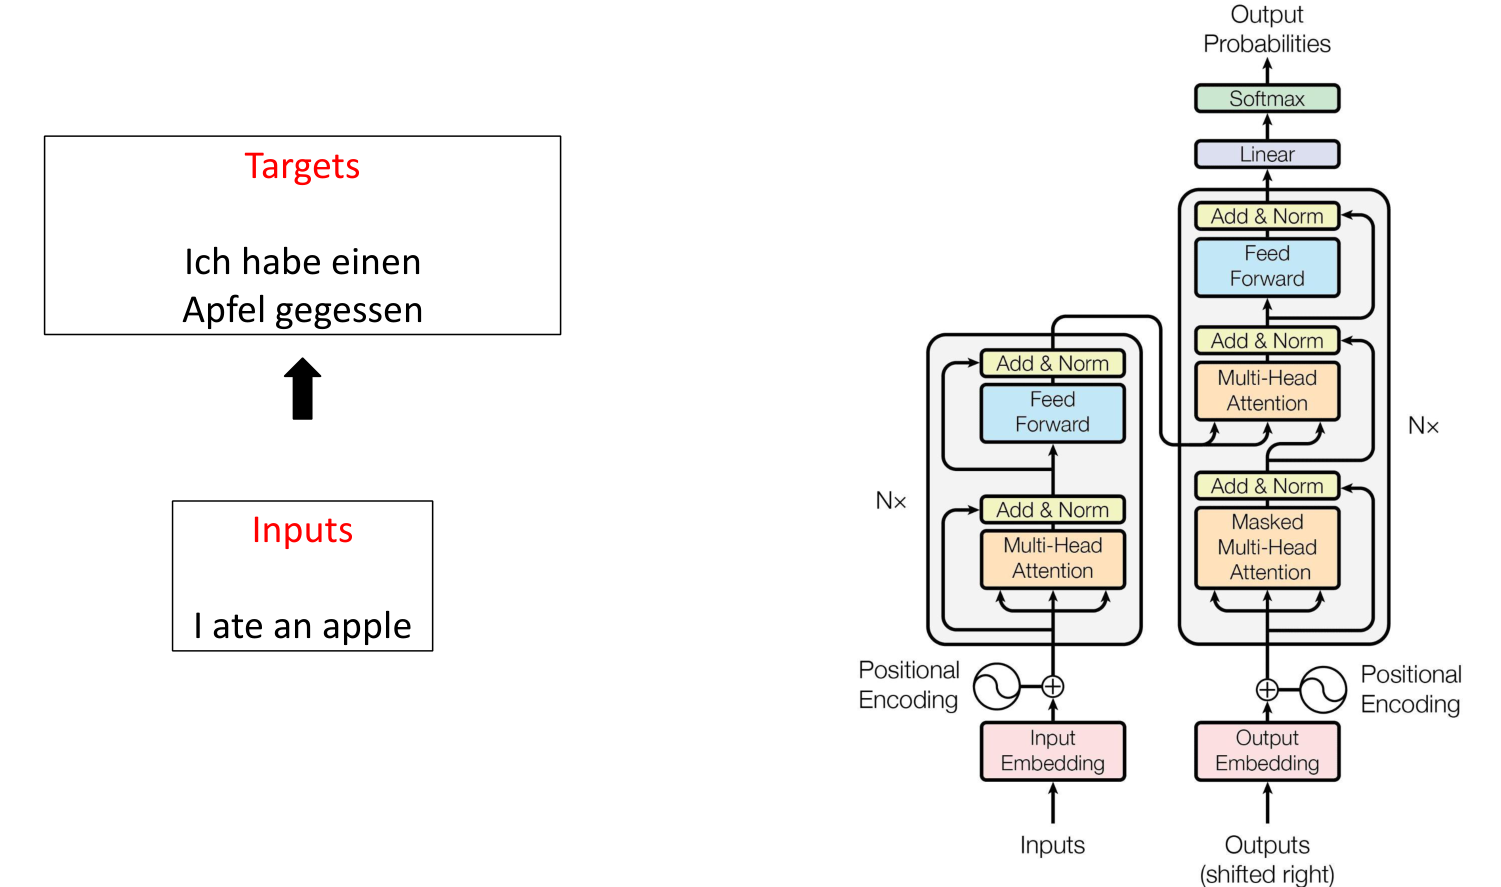
\includegraphics[width=0.60\paperwidth,height=0.60\paperheight,keepaspectratio]{images/large-language-models/llm_translation_inputs_targets.png}

  {\scriptsize Source: CMU 11-785 (Spring 2024), Lecture 19: Transformers and Newer Architectures, slide~7; architecture panel: Vaswani et al., NeurIPS 2017, Fig.~1.}
\end{frame}


\begin{frame}{Inputs}
  \centering
  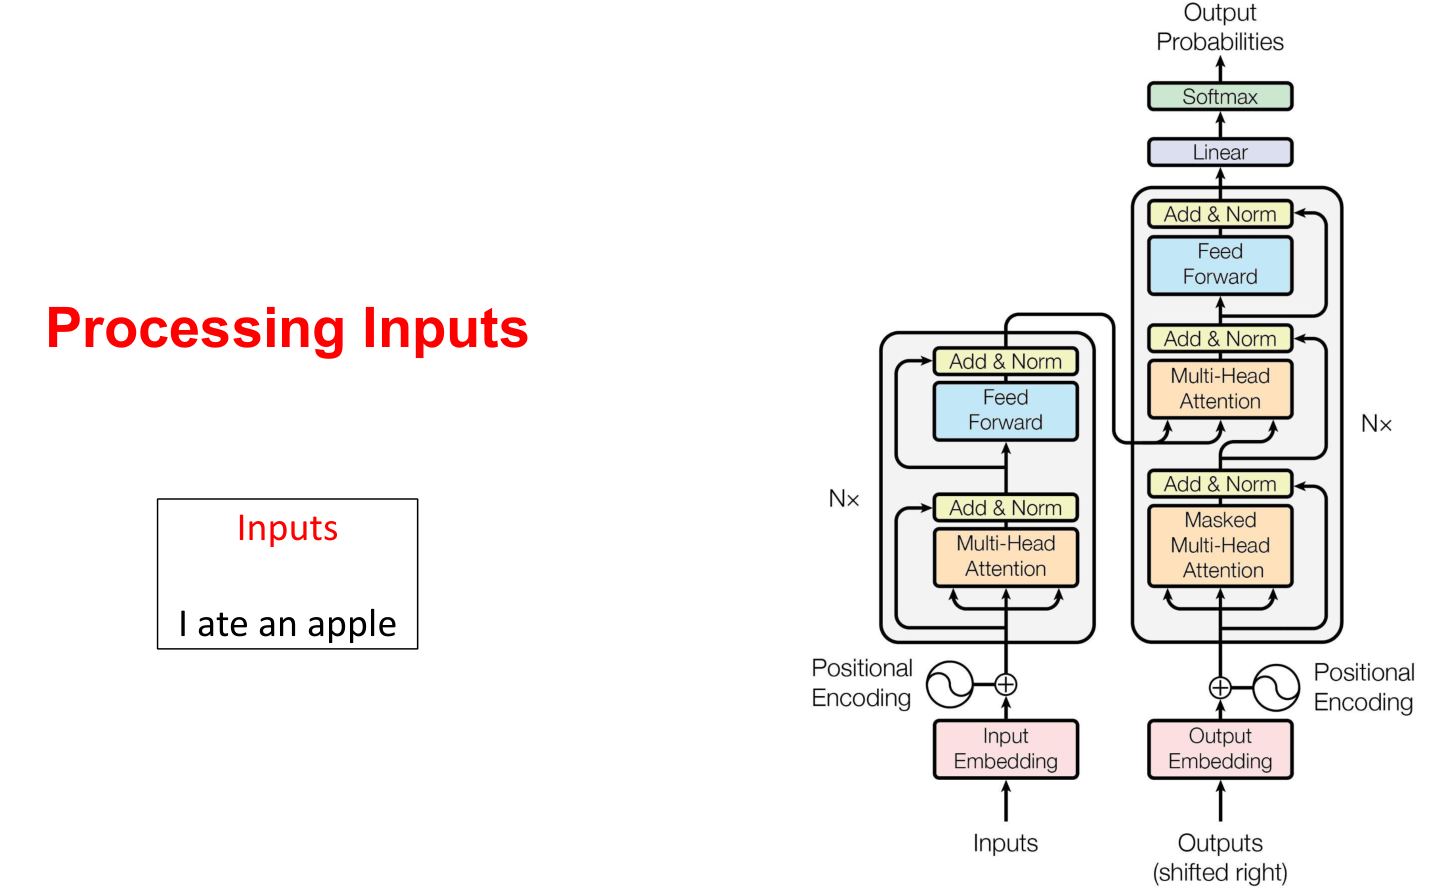
\includegraphics[width=0.60\paperwidth,height=0.60\paperheight,keepaspectratio]{images/large-language-models/llm_processing_inputs_transformer.png}

  {\scriptsize Source: CMU 11-785 (Spring 2024), Lecture 19: Transformers and Newer Architectures, slide~8; architecture panel: Vaswani et al., NeurIPS 2017, Fig.~1.}
\end{frame}

\begin{frame}{Tokenization}
  \centering
  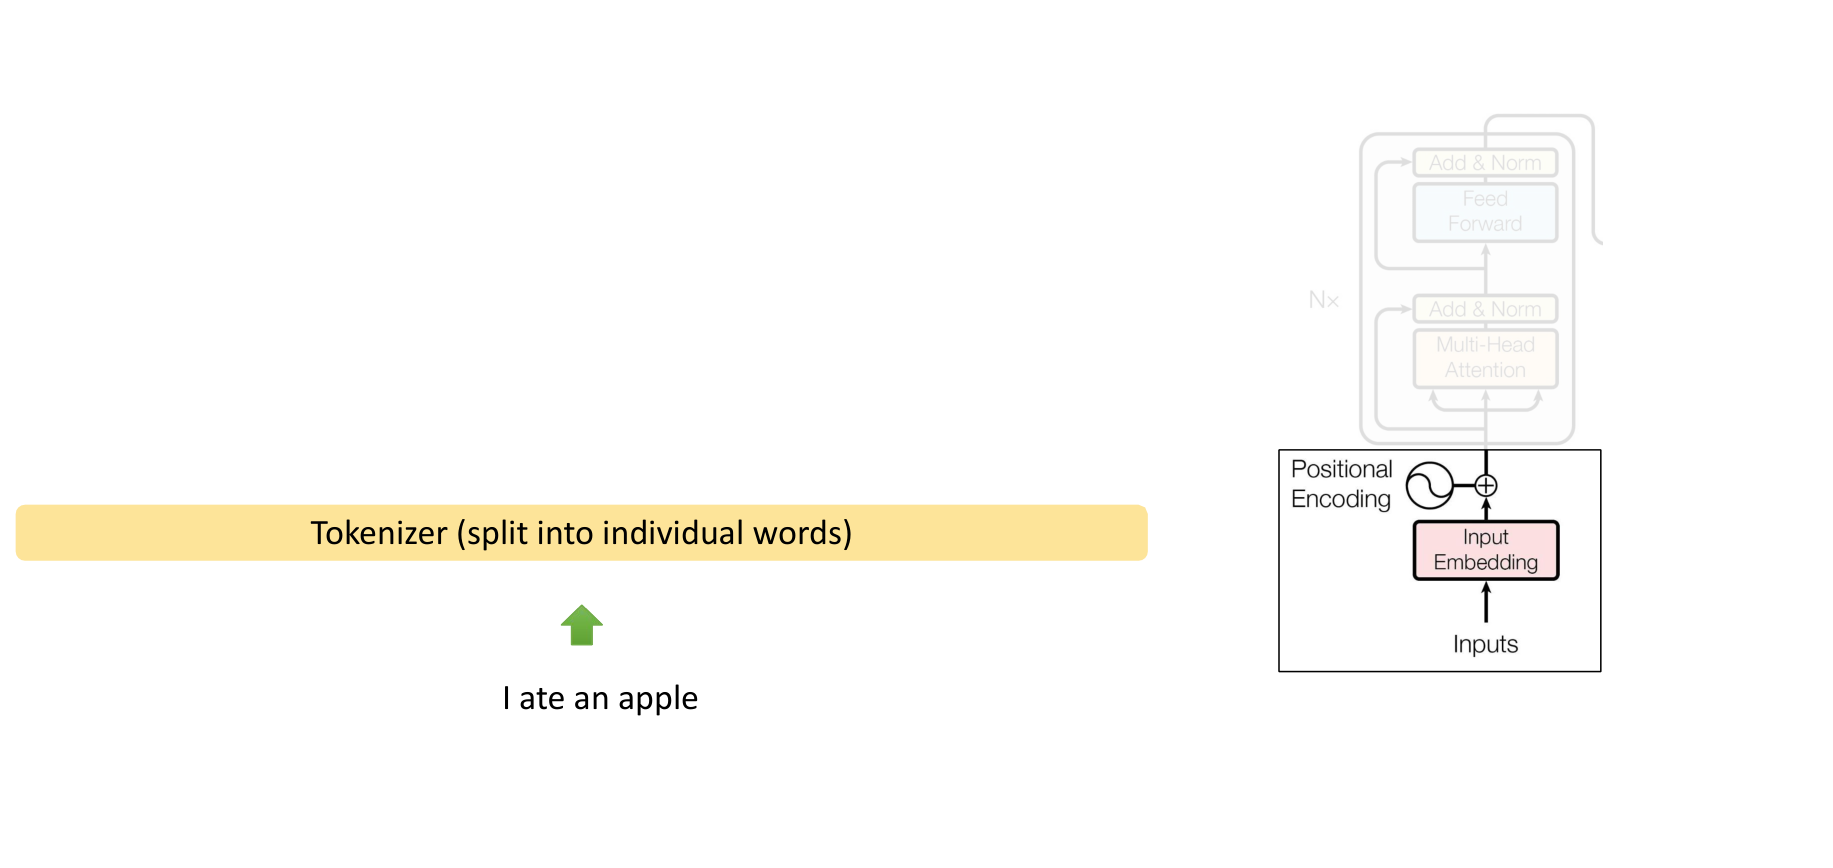
\includegraphics[width=0.8\paperwidth,height=0.70\paperheight,keepaspectratio]{images/large-language-models/llm_word_tokenizer_step.png}

  {\scriptsize Source: CMU 11-785 (Spring 2024), Lecture 19: Transformers and Newer Architectures, slide~9; architecture panel: Vaswani et al., NeurIPS 2017, Fig.~1.}
\end{frame}

\begin{frame}{Tokenization}
  \centering
  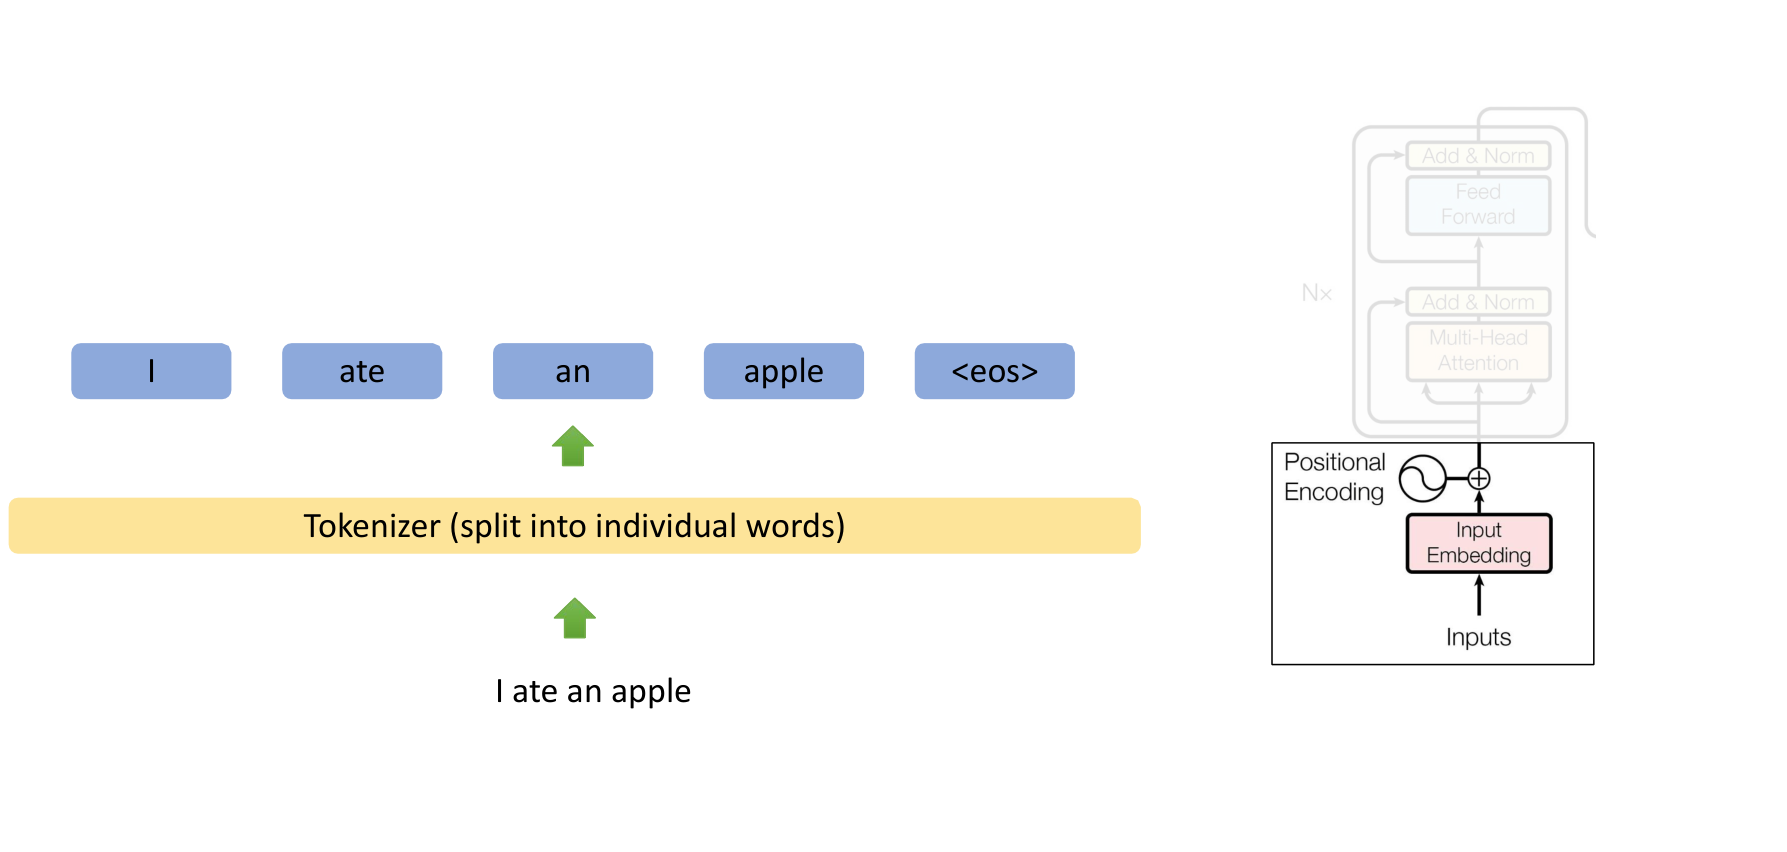
\includegraphics[width=0.8\paperwidth,height=0.70\paperheight,keepaspectratio]{images/large-language-models/llm_word_tokenizer_tokens.png}

  {\scriptsize Source: CMU 11-785 (Spring 2024), Lecture 19: Transformers and Newer Architectures, slide~10; architecture panel: Vaswani et al., NeurIPS 2017, Fig.~1.}
\end{frame}
